\documentclass{article}

\usepackage[margin=1in]{geometry}
\usepackage{booktabs}
\usepackage{graphicx}
\usepackage{amsmath}
\usepackage{hyperref}
\usepackage{xurl}
\usepackage{xcolor}
\usepackage{enumitem}

\definecolor{bestred}{HTML}{C62828}
\definecolor{secondblue}{HTML}{1565C0}
\newcommand{\best}[1]{\textcolor{bestred}{\textbf{#1}}}
\newcommand{\second}[1]{\textcolor{secondblue}{\underline{#1}}}

\title{A Benchmark and Polysaccharide-Specific Core Representation for Multi-label Structure-Function Prediction of Natural Polysaccharides}
\author{Qiang Xia\\Zhejiang Tea Group}
\date{}

\begin{document}
\maketitle

\begin{abstract}
Natural polysaccharides are increasingly studied for antioxidant, immunomodulatory, antitumor, and metabolic regulatory activities, yet machine learning for polysaccharide structure-function prediction remains underdeveloped. A major reason is that existing carbohydrate machine learning tools are largely glycan-centric, whereas natural polysaccharides are typically described by incomplete but heterogeneous structural evidence such as monosaccharide composition, linkage patterns, branching information, and molecular-weight ranges. We therefore build a practical benchmark for multi-label function prediction from public polysaccharide resources and examine which structural signals are actually useful under current public-data conditions. Starting from public-site DoLPHiN ingestion and a filtered benchmark of 4,121 records with 18 function labels, we reproduce classical, sequence, and graph baselines and establish a tuned logistic baseline as a strong sparse anchor. We then test a family of structure-aware extensions and find that the most stable conclusion is not that a new model decisively wins, but that a small set of structured features consistently carries the useful signal. Under a fixed random split, a compact polysaccharide-specific core representation that encodes molecular-weight buckets, branching availability, and residue-set composition improves macro-F1 from 0.2610 to 0.2678. However, under a stricter DOI-grouped split, the tuned logistic anchor remains stronger, indicating that the apparent gain is split-sensitive rather than robustly general. Paired bootstrap analysis further shows that the random-split gain is not statistically decisive. Controlled ablations nevertheless give a clear component-level empirical result: molecular-weight and residue features are the dominant contributors, branching provides a smaller positive effect, and several superficially plausible features are neutral or harmful. These results establish a reproducible benchmark, identify a strong sparse baseline, and clarify which structural signals are currently most useful within the present benchmark and preprocessing regime.
\end{abstract}

\section{Introduction}
\label{sec:intro}

Natural polysaccharides are multifunctional macromolecules associated with antioxidant, immunomodulatory, antitumor, anti-inflammatory, and metabolic regulation activities. The recent release of domain resources such as DoLPHiN makes it feasible to aggregate structural descriptors and reported health functions for thousands of natural polysaccharides, creating a realistic opportunity for data-driven prediction rather than purely narrative structure--function analysis. However, this opportunity is still technically immature. In contrast to proteins or small molecules, polysaccharides are rarely represented by a single clean sequence or graph. Instead, available descriptions are often heterogeneous and partially incomplete, combining monosaccharide composition, glycosidic linkages, branching descriptions, modifications, organism source, and approximate molecular-weight ranges.

This representation mismatch creates a practical challenge for machine learning. Existing carbohydrate machine learning has made real progress on glycans, including graph-based modeling and reusable software ecosystems, but these tools are largely built around glycan settings where sequence or graph structure is the primary object of analysis. Natural polysaccharide records are structurally broader and noisier. A direct transfer of glycan-centric representations therefore risks missing the signals that are most accessible in current polysaccharide databases. At the same time, claiming a large end-to-end foundation-model solution at this stage would be premature because benchmark construction, reproducible baselines, and component-level signal validation are still incomplete.

A second complication is semantic rather than architectural. In public resources such as DoLPHiN, function labels are inherited from what has been reported in the literature. The absence of a label therefore does not necessarily mean the polysaccharide truly lacks that function; it may simply be untested or unreported. The present task should therefore be read as weakly supervised multi-label prediction with positive-and-unlabeled characteristics, not as a fully observed true-negative classification problem \cite{jain2016weaklysupervised,li2022pu}.

This paper takes a narrower and more defensible position. We first construct a practical supervised benchmark from public polysaccharide resources, starting with full public-site ingestion of DoLPHiN and using CSDB only as an engineering stress-test source rather than as an equal supervised source. We then reproduce a set of classical, sequence, and graph baselines under fixed evaluation protocols, and identify a tuned logistic model as a strong and stable baseline. Our central insight is not that a new architecture clearly solves the task, but that the first reliable progress comes from understanding what the benchmark actually supports: a strong sparse anchor, a modest random-split gain from structured feature augmentation, and clear ablation evidence about which polysaccharide-specific signals matter.

Our contributions are summarized as follows:
\begin{itemize}[leftmargin=*,nosep]
\item We build a reproducible benchmark construction and baseline pipeline for multi-label polysaccharide structure--function prediction from public resources.
\item We show that a tuned sparse logistic baseline is a strong anchor on this benchmark, and that a compact polysaccharide-specific feature augmentation yields only a modest, split-sensitive gain rather than a uniformly robust improvement.
\item We use controlled ablations to show that molecular-weight and residue-set features are the dominant contributors, branching provides a smaller positive effect, and several plausible feature families are weak or harmful.
\end{itemize}

We deliberately limit our claim scope to current single-source supervised prediction and do not overclaim cross-source biological generalization, because the currently ingested CSDB slice is not label-aligned with the main task.

\section{Related Work}
\label{sec:related}

\paragraph{Polysaccharide data resources.}
DoLPHiN provides a database centered on structural and functional properties of natural polysaccharides with reported health benefits, making it a natural starting point for supervised polysaccharide prediction \cite{xin2025dolphin}. CSDB, by contrast, is a broader curated carbohydrate structure resource with deeper structural coverage for bacterial, fungal, and plant glycans \cite{toukach2022csdb}. At the broader glycoinformatics infrastructure level, GlyTouCan has played an important role as an interoperable glycan repository and accessioning system for heterogeneous glycan records \cite{tiemeyer2017glytoucan,fujita2021glytoucan3}. These resources are complementary, but they are not interchangeable for supervised function prediction. Our work builds operationally on both DoLPHiN and CSDB while explicitly recognizing that only the DoLPHiN-derived subset is currently suitable as the main supervision source for the present task.

\paragraph{Glycan machine learning.}
Recent glycan machine learning work has shown that carbohydrate-specific inductive biases matter. SweetNet demonstrated that graph convolutional neural networks are well matched to glycans because they directly model branching and nonlinear structure \cite{burkholz2021sweetnet}. Related work has also expanded glycan-focused machine learning into interaction prediction and broader deep-learning workflows, as exemplified by LectinOracle and other glycobiology-oriented computational resources \cite{lundstrom2022lectinoracle,bojar2021deeplearningresources}. This line of work motivates our general emphasis on structure-aware representation. However, our setting differs from glycan-focused prediction because natural polysaccharide records are often only partially graph-ready and are frequently reported through mixed textual and tabular evidence.

\paragraph{Practical glycobioinformatics tooling.}
Toolkits such as glycowork have lowered the barrier to glycan data analysis, representation engineering, and machine learning \cite{thomes2021glycowork}. At the representation-conversion layer, systems such as GlyLES further highlight the practical importance of standardizing carbohydrate encodings before downstream modeling \cite{joeres2023glyles}. We build on the broader lesson of this literature, namely that generic sequence or bag-of-words treatment is often insufficient for carbohydrate data. Our contribution is narrower than proposing a universal carbohydrate architecture. Instead, we identify which structured signals are already reliable enough to improve multi-label function prediction for natural polysaccharides under current public-data conditions.

\paragraph{Weak supervision, evaluation, and leakage risk.}
The supervision regime in this problem is also closer to curated weak supervision than to fully observed labeling. Prior biomedical information extraction work has shown that curated databases can be a useful supervision source while still carrying systematic incompleteness and reporting bias \cite{jain2016weaklysupervised}. In bioinformatics more broadly, positive-unlabeled learning has become a standard way to reason about settings in which observed positives are mixed with unobserved rather than confirmed negatives \cite{li2022pu}. This matters for evaluation as well as modeling: in multi-label classification, metric rankings can change materially depending on whether one emphasizes F-measure-style balanced recovery or stricter exact-label agreement \cite{pillai2017fmeasure}. Finally, recent work on leakage in machine-learning-based science reinforces the need to supplement random splits with grouped or source-aware reassessment when records can share paper-specific or reporting-specific artifacts \cite{kapoor2023leakage}. These considerations shape both our claim scope and our revised evaluation protocol.

\section{Method}
\label{sec:method}

Given a natural polysaccharide record with structural descriptors and metadata, our goal is to predict a set of functional labels from a fixed label vocabulary. Each record is represented by a canonical textual description together with fields such as monomer composition, linkage, branching, modification, molecular weight or molecular-weight range, and organism source. The target is a multi-label set over 18 retained biological function categories. Figure~\ref{fig:pipeline} summarizes the pipeline from raw public ingestion to the final \texttt{poly-core v1} method.

\begin{figure}[t]
\centering
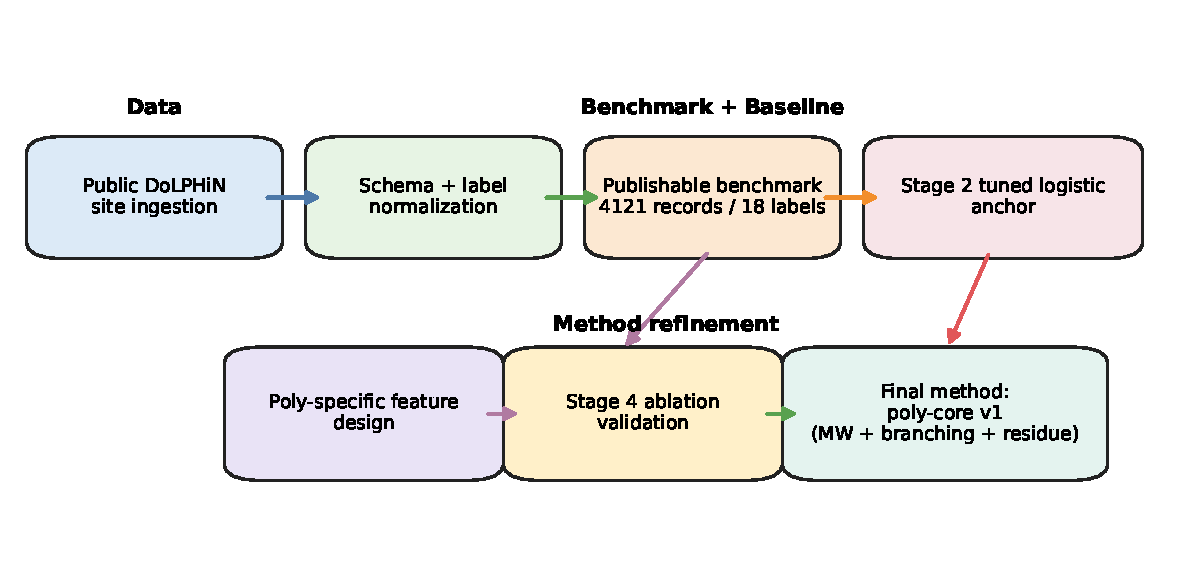
\includegraphics[width=0.98\linewidth]{figures/figure1_pipeline.pdf}
\caption{Overview of the benchmark construction and \texttt{poly-core v1} pipeline. Public-site ingestion is followed by schema and label normalization, benchmark filtering, fixed split generation, sparse-anchor training, and structured token augmentation.}
\label{fig:pipeline}
\end{figure}

\subsection{Benchmark Construction}
\label{sec:benchmark}

We construct the benchmark from public-site ingestion of DoLPHiN followed by schema normalization and label normalization. To obtain a stable supervised task, we remove \texttt{unknown} labels, retain only DoLPHiN as the supervision source, and keep only labels with global frequency of at least 20. The resulting benchmark contains 4,121 records and 18 function labels.

We intentionally separate benchmark construction from engineering stress testing. A second ingestion path from CSDB is useful for future cross-source work, but the currently available CSDB slice is structurally rich and label-poor relative to the supervised task. For that reason, CSDB is excluded from the main supervised benchmark and is not used to support the core empirical claim of this paper.

For the main benchmark split, we use a precomputed fixed partition with 2,472 training records, 824 validation records, and 825 test records. In the revised protocol, Stage 2--4 development decisions are made on the same fixed train/validation/test partition, with validation used for tuning and method selection and test reserved for final reporting only. This keeps later-stage comparisons attributable to controlled representation changes rather than split regeneration, while avoiding test-driven method selection.

Table~\ref{tab:dataset_stats} summarizes the main benchmark statistics. The filtered benchmark is label-sparse and field-imbalanced: records contain 1.56 labels on average, linkage is missing for most records, modification is effectively absent after filtering, and all retained records have \texttt{evidence\_type = unknown}. These properties reinforce that the task is best interpreted as structured weak supervision over heterogeneous literature-derived records rather than as a clean fully supervised molecular benchmark.

\subsection{Tuned Sparse Baseline}
\label{sec:baseline}

Our baseline starts from a simple but strong sparse representation. For each record, we concatenate the canonical representation, monomer composition, linkage, branching, modification, molecular-weight field, source database, and organism source into a lightweight feature string. This string is vectorized with a count-based vocabulary and fed into a one-vs-rest logistic regression classifier. In the revised evaluation protocol, this tuned sparse model is treated as the main anchor rather than as a disposable baseline to be surpassed at all costs.

Stage 2 tuning shows that this baseline is deterministic on the fixed split and benefits materially from reduced regularization and balanced class weighting. The strongest tuned configuration uses \texttt{C = 16.0} and \texttt{class\_weight = balanced}, and serves as the main comparison anchor for the rest of the paper.

\subsection{Polysaccharide-Specific Structural Representation}
\label{sec:polycore}

A remaining challenge is that the tuned sparse baseline treats many polysaccharide-specific cues as raw text rather than as normalized signals. Natural polysaccharide records repeatedly expose three high-value cues that are only weakly standardized in the raw text: coarse molecular-weight scale, whether branching information is available, and which residue families are present. These cues are common enough to be extracted reliably, but structured enough to be diluted when left entirely to generic tokenization.

To address this mismatch, we derive a compact token set from the existing structured fields. First, we parse molecular-weight fields into coarse buckets. Second, we encode whether branching information is available. Third, we derive residue-family tokens from monomer composition, linkage, branching, and canonical structural strings, producing markers such as glucose-, galactose-, arabinose-, mannose-, rhamnose-, xylose-, and uronic-acid-related residue presence, together with a residue-diversity signal. These tokens are appended to the tuned baseline feature text and processed by the same logistic classifier.

This design is intentionally modest. It does not attempt to reconstruct a complete carbohydrate graph from partially specified text, and it does not assume explicit evidence-level annotations that the current benchmark does not contain. Instead, it encodes the most reliable structural regularities that recur in public polysaccharide records and that can be defended by controlled ablation.

\subsection{From Poly-feature-only to Poly-core v1}
\label{sec:refinement}

Our first Stage 3 representation was intentionally broader and included evidence-proxy features, sample weighting by structural completeness, source-kingdom tokens, modification tokens, and composition-count tokens. This broader version produced a small gain over the tuned logistic baseline, but Stage 4 ablation revealed that the useful signal was concentrated in a smaller subset of components.

The final method, \texttt{poly-core v1}, therefore keeps only the three ablation-supported families: molecular-weight buckets, branching tokens, and residue-set tokens. It removes weak evidence-proxy features, sample weighting, source-kingdom context, modification features, and composition-count tokens. This simplification improves the final result and keeps the method aligned with the evidence actually supported by the experiments.

A full artifact checklist, benchmark-statistics note, split summary, and token-level reproducibility note are prepared separately as supplementary material so that the main paper can stay focused on the benchmark and method claim.

\section{Experiments}
\label{sec:exp}

\subsection{Experimental Setup}

The main supervised benchmark is \texttt{dataset\_publishable\_supervised\_v1}, which contains 4,121 DoLPHiN-derived records and 18 canonical function labels. We evaluate under a fixed random split protocol and report macro-F1 as the primary metric because the label distribution is highly imbalanced. We also report exact match ratio as a stricter secondary metric. Because the label space is weakly supervised and positive-unlabeled in character, these metrics should be interpreted as comparative ranking tools under a fixed protocol rather than as direct estimates of absolute biological truth. In particular, exact match is highly sensitive to over- and under-predicting the full label set for each record, whereas macro-F1 better reflects whether rare labels are recovered at all; the two metrics therefore need not rank sparse baselines in the same order \cite{pillai2017fmeasure}.

We compare trivial, classical, sequence, graph, and additional simple sparse baselines, including a majority predictor, untuned logistic regression, random forest, TF-IDF logistic regression, linear SVM, a lightweight sequence n-gram model, a lightweight transformer baseline implemented with native PyTorch modules, and a graph GCN baseline. After Stage 2 tuning, logistic regression with \texttt{C = 16.0} and balanced class weighting becomes the main anchor. All Stage 2--4 runs reuse the same fixed train/validation/test partition, and the reported multi-seed runs are deterministic in this setting, so the final comparison reflects controlled representation differences rather than optimization variance.

The benchmark split contains 2,472 training records, 824 validation records, and 825 test records. The benchmark is generated by retaining only DoLPHiN-derived supervision, removing \texttt{unknown} labels, and keeping labels with global frequency of at least 20. This fixed split is intentionally reused across Stage 2, Stage 3, and Stage 4 so that each later-stage comparison isolates representation or configuration changes rather than split-induced variance; within that fixed split, validation is the development partition and test is the final hold-out partition.

\paragraph{Implementation details.}
The tuned logistic anchor uses count-vectorized feature text with a token pattern that preserves alphanumeric, equality, and hyphen-delimited tokens, \texttt{min\_df = 1}, no vocabulary cap, \texttt{C = 16.0}, \texttt{class\_weight = balanced}, and one-vs-rest logistic regression with the \texttt{liblinear} solver. On the fixed training split, this yields a vocabulary of 6,255 tokens. The final \texttt{poly-core v1} method keeps the same classifier and augments the input text with only three structured token families: molecular-weight buckets (\texttt{<10 kDa}, \texttt{10--100 kDa}, \texttt{100 kDa--1 MDa}, \texttt{$\geq$1 MDa}, or unknown), branching-presence tokens, and residue-set tokens derived from the canonical structure, monomer composition, linkage, and branching fields. It does not use evidence-proxy features, sample weighting, source-kingdom features, modification tokens, or coarse composition-count tokens. This design choice follows directly from the Stage 3 and Stage 4 ablation results.

\begin{table}[t]
\centering
\caption{Main benchmark statistics for the filtered DoLPHiN-derived supervised dataset. Missing-rate values are computed after filtering into the 4,121-record benchmark.}
\label{tab:dataset_stats}
\begin{tabular}{lc}
\toprule
Statistic & Value \\
\midrule
Records & 4,121 \\
Labels retained & 18 \\
Average labels per record & 1.56 \\
Median labels per record & 1 \\
Canonical representation missing rate & 0.0\% \\
Monomer composition missing rate & 2.4\% \\
Linkage missing rate & 80.9\% \\
Branching missing rate & 0.0\% \\
Modification missing rate & 100.0\% \\
MW/range missing rate & 26.6\% \\
Organism-source missing rate & 0.0\% \\
DOI missing rate & 0.1\% \\
Retained evidence type & unknown only \\
\bottomrule
\end{tabular}
\end{table}

\subsection{Main Results}

Table~\ref{tab:main_results} and Figure~\ref{fig:main_results} report the random-split comparison. To avoid an unfair reading of the table, we separate it conceptually into two parts: reproduced baseline families and the tuned logistic anchor plus proposed methods. We did not run a full Stage 2 hyperparameter search for every baseline family, so the tuned logistic result should be interpreted as the strongest stable anchor rather than as proof that all other model families are fully optimized. The reproduced baselines should therefore be read as breadth-of-family references, whereas the tuned logistic row is the paper's explicit optimization anchor. Based on these results, we make four observations:
\begin{itemize}[leftmargin=*,nosep]
\item \textbf{The benchmark is nontrivial.} The majority baseline reaches only 0.0397 macro-F1, while untuned logistic regression improves to 0.1580. The majority exact-match value remains comparatively high because many records carry only one retained label and the label space is sparse. Even under that favorable exact-match condition, prior frequency alone is inadequate for balanced recovery, whereas a sparse textual view of structure already contains predictive signal.
\item \textbf{Tuning matters more than early architectural novelty.} Stage 2 increases the logistic anchor from 0.1580 to 0.2610 macro-F1, largely through weaker regularization and balanced class weighting. This justifies using tuned logistic regression as the main anchor for method development.
\item \textbf{Additional sparse baselines matter, but they change the ranking by metric.} TF-IDF logistic regression and linear SVM do not beat the tuned count-based logistic anchor on macro-F1, but they achieve the strongest exact-match scores among the added simple sparse baselines. This confirms that the benchmark supports multiple competitive sparse references and that metric choice materially changes which simple model looks strongest.
\item \textbf{The final representation gives only a modest random-split gain.} \texttt{poly-core v1} improves macro-F1 to \best{0.2678}, exceeding the tuned logistic anchor at \second{0.2610}. However, this gain is small, its paired bootstrap confidence interval crosses zero, and the paired bootstrap p-value is 0.448. The gain also does not persist under the stricter grouped-split setting introduced below. We therefore treat it as a promising but split-sensitive result rather than as a decisive model win. Its exact match is not the best value in the table, which reinforces that our claim is specifically about balanced multi-label recovery under macro-F1 rather than about optimizing the strictest all-label metric.
\end{itemize}

\begin{table}[t]
\centering
\caption{Main comparison on \texttt{publishable\_supervised\_v1}. Upper block: reproduced baseline families under a shared fixed protocol without exhaustive family-specific tuning. Lower block: the explicitly tuned logistic anchor and the proposed method variants. Note that macro-F1 and exact match emphasize different failure modes in this weakly supervised multi-label setting, so the strongest model need not be the same under both metrics. \best{Red}: best, \second{blue}: second best.}
\label{tab:main_results}
\begin{tabular}{lcc}
\toprule
Method & Macro-F1 $\uparrow$ & Exact Match $\uparrow$ \\
\midrule
Majority & 0.0397 & 0.2776 \\
Logistic (untuned) & 0.1580 & 0.2848 \\
Random Forest & 0.1752 & \best{0.3127} \\
TF-IDF + Logistic & 0.2514 & 0.2897 \\
Linear SVM & 0.2521 & \second{0.2921} \\
Sequence n-gram & 0.2035 & 0.2824 \\
Sequence Transformer & 0.0397 & 0.2776 \\
Graph GCN & 0.2103 & 0.1442 \\
\midrule
Logistic (tuned) & \second{0.2610} & 0.2606 \\
Poly-feature-only v1 & 0.2654 & 0.2582 \\
Poly-core v1 & \best{0.2678} & 0.2570 \\
\bottomrule
\end{tabular}
\end{table}

\begin{figure}[t]
\centering
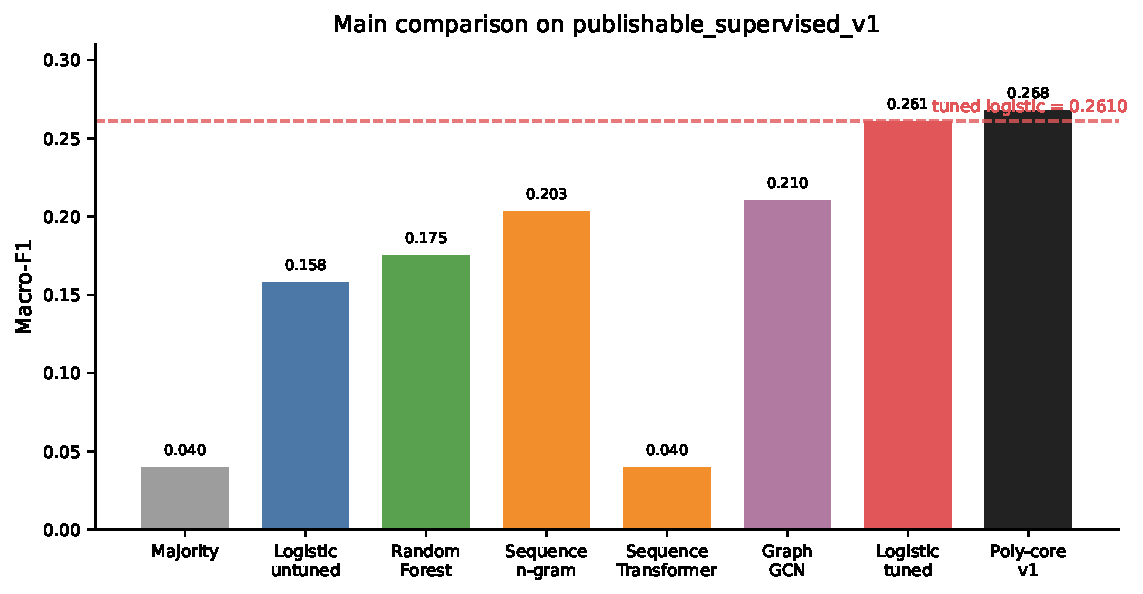
\includegraphics[width=0.92\linewidth]{figures/figure2_main_results.pdf}
\caption{Main comparison on the \texttt{publishable\_supervised\_v1} benchmark. Among the reproduced untuned methods, linear SVM is the strongest macro-F1 baseline, while random forest gives the best exact match. The tuned logistic anchor remains the strongest tuned sparse reference, and the final \texttt{poly-core v1} method gives the best macro-F1 under the fixed random-split protocol.}
\label{fig:main_results}
\end{figure}

\subsection{Grouped-Split and Bootstrap Reassessment}

To address the risk that a fixed random split overestimates generalization, we added a deterministic DOI-grouped split in which all records sharing the same DOI are kept in the same partition. This split removes a major source of near-duplicate leakage through paper-specific phrasing and reporting patterns. We also evaluate the tuned logistic anchor and \texttt{poly-core v1} under a development protocol that uses validation for method selection and reports test only once for the final frozen comparison. This grouped reassessment is motivated by the broader concern that unnoticed leakage can materially inflate scientific model claims even when the underlying implementation is otherwise correct \cite{kapoor2023leakage}.

Table~\ref{tab:robustness_results} summarizes the revised picture. Under the random split, \texttt{poly-core v1} still shows a small positive delta over the tuned logistic anchor on the test partition. However, paired bootstrap analysis yields a 95\% confidence interval of \([-0.0115, 0.0260]\) and a two-sided bootstrap p-value of 0.448, so the random-split gain is not statistically decisive. Under the DOI-grouped split, the direction reverses: tuned logistic reaches 0.1250 macro-F1 on the grouped test partition, whereas \texttt{poly-core v1} reaches 0.1140. The corresponding bootstrap interval for the difference is \([-0.0254, 0.0020]\) with p = 0.108. In other words, the current feature augmentation is informative for ablation and representation analysis, but not yet robust enough to support a strong grouped-generalization claim.

Per-label analysis reinforces the same conclusion. On the random split, the aggregate macro-F1 gain is concentrated in a small subset of labels such as \textit{antimicrobial}, \textit{neuroprotective}, and \textit{organ-protective} prediction rather than being broadly uniform. Under the DOI-grouped split, some labels degrade sharply, most notably \textit{antiaging}. We therefore treat the feature augmentation as a label-sensitive and split-sensitive modification, not as a universally stronger classifier. The additional TF-IDF and SVM baselines point in the same direction: simple sparse alternatives can improve exact match without improving macro-F1, so metric trade-offs must be read explicitly rather than collapsed into a single notion of ``best''.

Qualitative case studies show the same pattern at the record level: \texttt{poly-core v1} can recover missing labels or prune false positives on selected examples, but it also introduces grouped-split failures where the tuned logistic anchor remains correct. This makes the method more useful as a probe for feature relevance than as a settled replacement for the sparse anchor.

\begin{table}[t]
\centering
\caption{Revised robustness summary for the tuned logistic anchor and \texttt{poly-core v1}. Validation is used for development; test is used once for final reporting. Reported confidence intervals are paired bootstrap intervals for the macro-F1 difference \texttt{poly-core v1} minus tuned logistic on the test partition.}
\label{tab:robustness_results}
\begin{tabular}{lcccc}
\toprule
Split & Logistic val & Poly-core val & Logistic test & Poly-core test \\
\midrule
Random & 0.3143 & 0.3152 & 0.2610 & 0.2678 \\
DOI-grouped & 0.1189 & 0.1218 & \best{0.1250} & 0.1140 \\
\bottomrule
\end{tabular}

\vspace{0.3em}
\begin{tabular}{lccc}
\toprule
Test comparison & $\Delta$ Macro-F1 & 95\% CI & p-value \\
\midrule
Random split & +0.0068 & [-0.0115, 0.0260] & 0.448 \\
DOI-grouped split & -0.0110 & [-0.0254, 0.0020] & 0.108 \\
\bottomrule
\end{tabular}
\end{table}

\subsection{Stage-wise Method Development}

The experiment pipeline clarifies how the final result emerged. Stage 1 established executable baselines across classical, sequence, and graph families. Stage 2 showed that tuned logistic regression was the strongest stable anchor. Stage 3 then tested whether a broad evidence-aware extension could improve over that anchor. It could not. The full evidence-aware variant underperformed the tuned logistic baseline, and its sub-variants revealed that weak evidence proxies and broad token augmentation were not the source of gain.

This negative result is informative and should be read as a scoped failure case rather than as a discarded implementation detail. The current supervised benchmark does not contain meaningful variation in explicit evidence-level annotation; all retained records carry \texttt{evidence\_type = unknown}. Therefore, a strong evidence-aware claim would be technically weak. The effective gain instead comes from a core structural representation that better matches the reporting style of natural polysaccharides, although the grouped-split reassessment shows that this gain is not yet robust enough to displace the tuned sparse anchor as the strongest overall conclusion.

\begin{table}[t]
\centering
\caption{Stage 3 method evolution under the same tuned logistic backbone. This table makes the failure-to-success trajectory explicit rather than leaving it implicit in the text.}
\label{tab:stage3_evolution}
\begin{tabular}{lc}
\toprule
Configuration & Macro-F1 $\uparrow$ \\
\midrule
Tuned logistic anchor & 0.2610 \\
Evidence-aware v1 (full) & 0.2579 \\
Weight-only variant & 0.2595 \\
Feature-only variant (poly + evidence tokens) & 0.2582 \\
Poly-feature-only v1 & 0.2654 \\
Poly-core v1 & \best{0.2678} \\
\bottomrule
\end{tabular}
\end{table}

\subsection{Ablation Study}

Table~\ref{tab:ablation} and Figure~\ref{fig:ablation} summarize the key ablations around the initial Stage 3 winner \texttt{poly-feature-only v1}. Based on these results, we make three observations:
\begin{itemize}[leftmargin=*,nosep]
\item \textbf{Molecular-weight buckets are the strongest component.} Removing MW tokens reduces macro-F1 from 0.2654 to 0.2461, the largest drop among all ablations.
\item \textbf{Residue-set tokens are also critical.} Removing residue tokens reduces macro-F1 to 0.2533, confirming that coarse residue-family composition provides important function-related signal.
\item \textbf{Not every engineered feature helps.} Branching remains a supported positive component, but modification and source-kingdom tokens are weak. Removing composition-count tokens actually improves performance, which allows us to simplify the method into the final \texttt{poly-core v1} configuration.
\end{itemize}

\begin{table}[t]
\centering
\caption{Ablation study around \texttt{poly-feature-only v1} (reference macro-F1 = 0.2654). Positive deltas indicate improvement after removing a component.}
\label{tab:ablation}
\begin{tabular}{lcc}
\toprule
Ablation & Macro-F1 $\uparrow$ & $\Delta$ vs. Reference \\
\midrule
Remove MW & 0.2461 & -0.0193 \\
Remove branching & 0.2598 & -0.0056 \\
Remove modification & 0.2619 & -0.0035 \\
Remove residue & 0.2533 & -0.0121 \\
Remove source kingdom & 0.2621 & -0.0033 \\
Remove composition terms & \second{0.2669} & \best{+0.0015} \\
\midrule
Poly-core v1 & \best{0.2678} & \second{+0.0024} \\
\bottomrule
\end{tabular}
\end{table}

\begin{figure}[t]
\centering
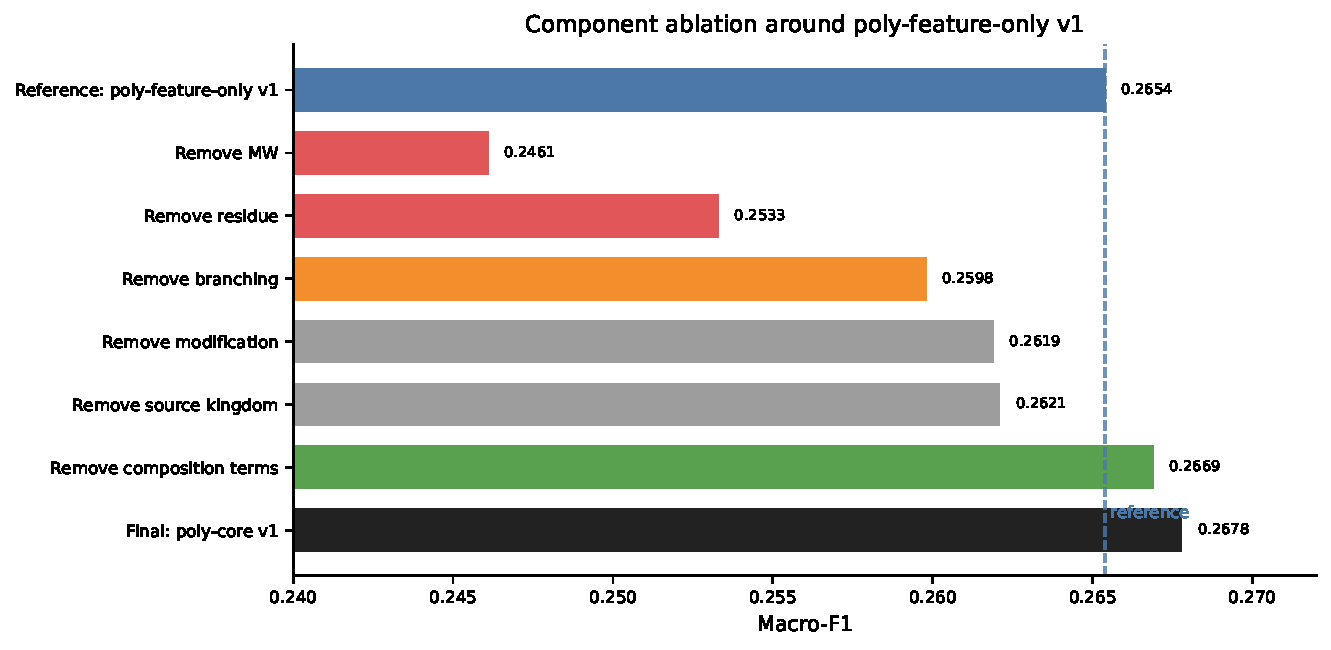
\includegraphics[width=0.92\linewidth]{figures/figure3_ablation.pdf}
\caption{Component ablation around \texttt{poly-feature-only v1}. Molecular-weight and residue features are the strongest positive contributors, while the coarse composition-count feature family is slightly harmful and is removed in the final method.}
\label{fig:ablation}
\end{figure}

\subsection{Stress-test and Scope Boundary}

We also built a merged \texttt{DoLPHiN + CSDB} pipeline and ran leave-one-source-out experiments as an engineering stress test. This pipeline is executable and useful for future work, but it should not be overinterpreted in the current paper. The present CSDB slice is structurally valuable but not label-aligned with the main supervised task, and training on it does not provide a fair biological test of function prediction generalization.

We therefore treat cross-source evaluation as a forward-looking stress-test result rather than as the main scientific evidence. This scope boundary keeps the paper centered on a benchmark claim that is genuinely supported by the available data.

\section{Conclusion}
\label{sec:conclusion}

We presented a reproducible benchmark and modeling pipeline for multi-label structure--function prediction of natural polysaccharides. Starting from public DoLPHiN ingestion and a filtered supervised benchmark, we reproduced a range of baseline families and established a tuned logistic regression anchor that is stronger than a naive reading of the problem might suggest. We then showed that a compact polysaccharide-specific structural representation can produce a modest random-split gain, while controlled ablations demonstrate that molecular-weight, residue-set, and branching features drive that gain.

The main scientific insight is narrower than our original Stage 3 hypothesis. On the current benchmark, the decisive contribution is not a universally stronger model, but a clearer understanding of what the benchmark supports: a strong sparse anchor, a split-sensitive structured augmentation, and a set of feature-level findings that remain interpretable under ablation. This narrower claim is also the more credible one: it identifies which signals are useful within the present benchmark and preprocessing regime, and avoids claiming more than the current public data can support.

\paragraph{Limitation.}
Our benchmark is intentionally conservative and single-source in its main supervised setting. Although we implemented a merged \texttt{DoLPHiN + CSDB} pipeline, the currently ingested CSDB slice is not label-aligned enough to support a strong cross-source supervised claim. In addition, explicit evidence-level annotations are largely unavailable in the retained supervised data, which limits the strength of any current evidence-aware modeling result. More fundamentally, the benchmark labels are literature-derived positives with unknown negatives, so the task is closer to weakly supervised or positive-unlabeled multi-label prediction than to fully observed classification \cite{li2022pu}. The revised DOI-grouped split also shows that the current feature augmentation does not yet deliver robust grouped generalization, even though it remains informative in random-split ablations; this is exactly the kind of fragility that grouped reassessment is meant to expose in leakage-prone scientific settings \cite{kapoor2023leakage}. Future work should therefore focus on better evidence annotation, stronger source alignment, more chemically faithful cross-database structural normalization, PU-aware evaluation and learning protocols, and grouped generalization tests rather than on scaling model size alone.

\paragraph{Reproducibility note.}
To reduce ambiguity between the benchmark claim and the engineering scaffold, we provide a supplementary reproducibility package that lists the exact benchmark artifact names, split statistics, tuned-anchor configuration, and final token-family definition used for \texttt{poly-core v1}. The project repository is available at \url{https://github.com/ShawnXiha/polysaccharide-function-benchmark}.

\bibliographystyle{plain}
\bibliography{references_poly_core_v1}

\end{document}
